% Created 2018-01-16 Tue 22:04
% Intended LaTeX compiler: pdflatex
\documentclass[11pt]{article}
\usepackage[utf8]{inputenc}
\usepackage[T1]{fontenc}
\usepackage{graphicx}
\usepackage{grffile}
\usepackage{longtable}
\usepackage{wrapfig}
\usepackage{rotating}
\usepackage[normalem]{ulem}
\usepackage{amsmath}
\usepackage{textcomp}
\usepackage{amssymb}
\usepackage{capt-of}
\usepackage{hyperref}
\usepackage{float}
\usepackage[margin=2cm]{geometry}
\date{\today}
\title{}
\hypersetup{
 pdfauthor={},
 pdftitle={},
 pdfkeywords={},
 pdfsubject={},
 pdfcreator={Emacs 25.3.1 (Org mode 9.1.3)}, 
 pdflang={English}}
\begin{document}


\section{Integrales Racionales}
\label{sec:org11ed78f}
Si \(P(x), Q(x)\) son dos polinomios, llamaremos a \(f(x) = \frac{P(x)}{Q(x)}\) una funcion racional.

Buscamos 
\[ 
\int f(x) dx
\]

\section{Integrales Utiles}
\label{sec:org16b4fb7}
Raiz Simple:
\[ 
\int \frac{A}{ax-b} dx = \frac{A}{a} \cdot ln(\lvert ax-b \rvert) + C 
\]
Raiz Multiple
\[ 
\int \frac{A}{(ax-b)^{n}} dx = A \cdot \frac{-1}{a(n-1)(ax-b)^{n-1}} + C
\]
Raiz Imaginaria (Termino con X) 
\[ 
\int \frac{Ax}{a^{2}x^{2} + b^{2}} dx = \frac{A}{2a^{2}} \cdot ln(\lvert a^{2}x^{2} + b^{2} \rvert)  + C 
\]
Raiz Imaginaria (Termino sin x)
\[ 
\int \frac{A}{a^{2}x^{2} + b^{2}} dx = \frac{A}{ab} \cdot arctan(\frac{ax}{b}) + C 
\]
\section{Resolucion}
\label{sec:org24a41e5}
\begin{enumerate}
\item Primero nos aseguramos que gr(Q(x)) > gr(P(x)), si no es asi podemos expresar \(f(x)\)  como \(S(x) + \frac{R(x)}{Q(x)}\) donde \(S(x)\) es el resultado de la division \(\frac{P(x)}{Q(x)}\) y R(x) el resto de la misma division. Como S(x) es un polinomio la integral es inmediata y \(\frac{R(x)}{Q(x)}\) pasa a ser nuestra integral racional.

\item Para facilitar el calculo de la integral, dividiremos a f(x) en suma de fracciones. Sea

\[
Q = (x-1)(x-2)^{2}(x^{2}+1) 
\]
Q es un polinomio de quinto grado con una raiz simple, una raiz multiple (doble) y una raiz imaginaria. 
Entonces 
\[
f(x) = \frac{P(x)}{Q(x)} = \frac{A}{x-1} + \frac{B}{x-2} + \frac{C}{(x-2)^{2}} + \frac{Dx + E}{x^{2} + 1}
\]
Esta igualdad se cumple para TODO valor de x, por lo tanto podemos sustituir tantos valores como incognitas y obtener las ecuaciones suficientes para resolver el problema. Para falicitar este calculo multiplicamos \(Q(x)\) a ambos lados y obtenemos:
\[
P(x) = \frac{A*Q(x)}{x-1} + \frac{B*Q(x)}{x-2} + \frac{C*Q(x)}{(x-2)^{2}} + \frac{(Dx + E)*Q(x)}{x^{2} + 1}
\]
Como Q(x) es el minimo comun divisor, se nos cancelaran todos los denominadores. Como estamos trabajando con polinomios, si sustituimos x por raices de \(Q(x)\) muchos terminos valdran 0. (en este caso probamos con 1 y 2. Necesitaremos 3 valores más ya que tenemos 5 incognitas) \\
Es importante ver que no estamos resolviendo por x, sino por ABCDE. Si tenemos estas 5 incognitas, independientemente del valor de x la igualdad se cumple.
\item Una vez encontrado las incognitas nuestro problema pasa a ser:
\end{enumerate}
\[
\int f(x) dx = \int\frac{P(x)}{Q(x)} dx = \int \frac{A}{x-1} + \frac{B}{x-2} + \frac{C}{(x-2)^{2}} + \frac{Dx + E}{x^{2} + 1} dx =
\]
\[
= \int \frac{A}{x-1} dx + \int \frac{B}{x-2} dx + \int \frac{C}{(x-2)^{2}} dx + \int \frac{Dx + E}{x^{2} + 1} dx =
\]
\[
= \int \frac{A}{x-1} dx + \int \frac{B}{x-2} dx + \int \frac{C}{(x-2)^{2}} dx + \int \frac{Dx}{x^{2} + 1} dx + \int \frac{E}{x^{2}+1} dx =
\]
\[
= Aln(\lvert x-1 \rvert) + Bln(\lvert x-2 \rvert) + C \cdot \frac{(x-2)^{-1}}{-1} + \frac{D}{2}*ln(\lvert x^{2}+1 \rvert) + E\cdot arctan(x) + Constante
\]
\section{Anexo}
\begin{figure}[H]
\centering
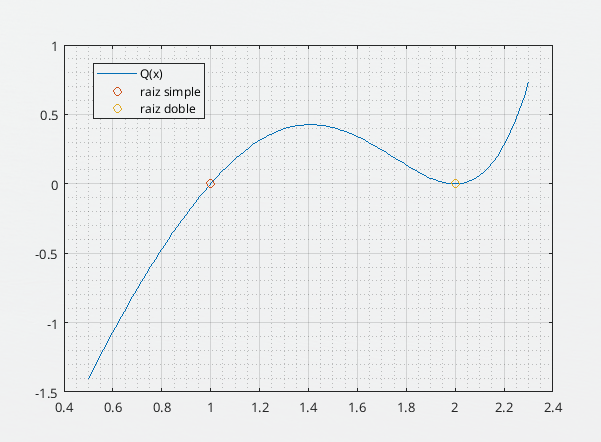
\includegraphics[width=.8\linewidth]{./Racional.png}
\caption{\label{fig:org83d02e0}
Grafica}
\end{figure}
\end{document}

